\section{Durchführung}
\label{sec:Durchführung}
\subsection{Versuchsaufbau}
\begin{figure}[h]
    \centering
    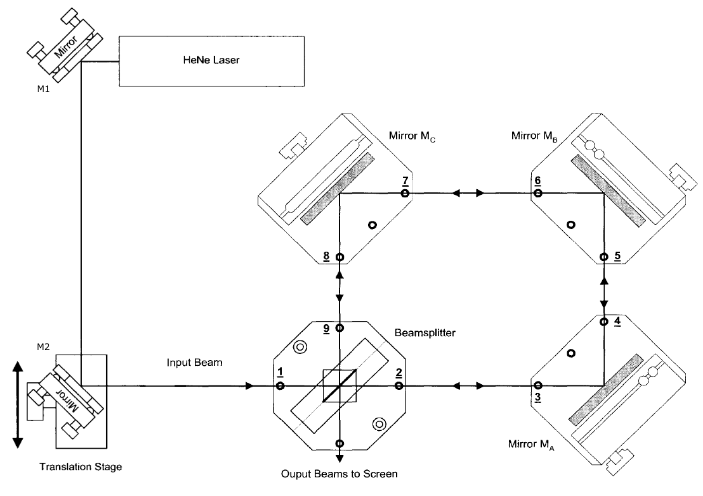
\includegraphics[width = \textwidth]{bild/Aufbau.png}
    \caption{Eine Darstellung des Versuchsaufbaus, der aus einem Sagnac-Interferometer besteht \cite{V64}.}
    \label{fig:Aufbau}
\end{figure}

\noindent
Der Versuch besteht aus einem Sagnac-Interferometer~\ref{fig:Aufbau},
in das ein Laser mit der Wellenlänge \SI{632.990}{\nano\metre} gestrahlt wird. 
Der Strahl trifft nach dem Verlassen des Interferometers auf einen 
\textit{polarizing beam splitter cube} (PBSC), 
der diesem in seine vertikale und horizontale Polarisationskomponenten zerlegt,
wodurch die Strahle eine Phasenverschiebung von 180° haben.
Diese werden auf zwei Dioden geleitet,
mit denen die Differenz der Photodiodenspannungen gemessen 
und auf dem Oszilloskop angezeigt wird.

\subsection{Justierung}%%%%%%%%%%%%%%%%%%%%%%%%%%%%%%%%%%%%%%%%%%%%%%%%%%%%%%%%%%%%%%%%%5555
Zuerst wird Sagnac-Interferometer justiert,
dass die den Strahle parallel zueinander verlaufen.
Er erste Strahl wird über zwei Spiegel so justiert,
dass dieser durch die zwei gegeben Lochblenden strahlt.
Mit den restlichen zwei Spiegeln wird der andere Strahl analog justiert.
 \newline
\noindent Ist alles korregt justiert,
sind die Strahlen nach dem Verlassen des Interferometers parallel und
treffen in einem Punkt auf den Schirm.
Bei konstruktiver Interferenz hat dieser Punkt seine maximale Helligkeit 
und bei destruktiver Interferenz verschwindet er.
Liegen die Strahlen nicht genau übereinander, sind Streifen zu sehen. 

\subsection{Kontrastbestimmung}%%%%%%%%%%%%%%%%%%%%%%%%%%%%%%%%%%%%%%%%%%%%%%%%%%%%%%%%%%%%%%%%%%%%%%%%%%%%%%%%
Der Kontrast wird in Abhängigkeit von der Polarisation gemessen,
indem vor dem Strahlteiler ein Polarisationsfilter gestellt wird.
Die Intensität der Interferenzmaxima/-minima wird für verschiedene Polarisationswinkel gemessen.
\newline \newline
\noindent Für die weiteren Messungen wird der größte Kontrast eingestellt.

\subsection{Messung des Brechungsindezes von Glas}%%%%%%%%%%%%%%%%%%%%%%%%%%%%%%%%%%%%%%%%%%%%%%%%%%%%
Zwei Glasplatten werden mit einem Winkel von $10\deg$ 
in die parallel laufenden Strahlen gestellt.
Die Platten werdem um $10\deg$ gedreht und die Anzahlder Interferenzminima  oder -maxima bestimmt
Diese Messung wird insgesamt 10 mal wiederholt.

\subsection{Messung des Brechungsindezes von Luft}%%%%%%%%%%%%%%%%%%%%%%%%%%%%%%%%%%%%%%%%%%%%%%%%%%%%%%%%%%%%%%%%%%%%%%%%%%%%%%%%%%%%%%%%%%%%%%%%%%%%%%%%%%%%%%%%%%%%%%%%%%%%%%%%%%%5
In einen der Strahlen wird eine auf 6 mbar evakuirte Gaszelle gestellt.
In 50 mbar-Schritten wird der Druck erhöht, bis wieder der Normaldruck ist
Währenddessen wird die Anzahl der Interferenzmaima notiert.
Die Messung wird 3 mal durchgeführt
\newline \newline
\noindent Die Messeung wird für eine weitere Gaszelle durchgeführt.
